\documentclass[11pt,letterpaper]{article}
\PassOptionsToPackage{hyphens}{url}
\usepackage[margin=.83in,top=.8in,bottom=.8in,headheight=15pt]{geometry}
\usepackage[T1]{fontenc}
\usepackage{lmodern,amsmath,amssymb,mathtools,bm,booktabs,array,graphicx,tikz}
\usetikzlibrary{arrows.meta,positioning,calc,decorations.pathreplacing,patterns}
\definecolor{ink}{HTML}{17344D}\definecolor{accent}{HTML}{087E8B}\definecolor{pale}{HTML}{EDF5F5}\definecolor{gold}{HTML}{AD6B19}
\providecommand{\dd}{\,\mathrm{d}}\providecommand{\R}{\mathbb{R}}
\providecommand{\E}{\mathbb{E}}\providecommand{\Var}{\operatorname{Var}}
\providecommand{\Cov}{\operatorname{Cov}}\providecommand{\diag}{\operatorname{diag}}
\providecommand{\norm}[1]{\left\lVert#1\right\rVert}
\providecommand{\abs}[1]{\left|#1\right|}
\usepackage{microtype,hyperref,fancyhdr,enumitem,amsthm,sectsty,needspace}
\allsectionsfont{\raggedright}
\hypersetup{colorlinks=true,linkcolor=ink,urlcolor=accent,pdfauthor={Zan Ahmad},pdftitle={Osmotic water transport and cell volume / Lecture notes}}
\setlength{\parindent}{0pt}\setlength{\parskip}{6pt}\linespread{1.07}
\setlist{itemsep=3pt,topsep=4pt,leftmargin=*}
\emergencystretch=2em\clubpenalty=10000\widowpenalty=10000
\pagestyle{fancy}\fancyhf{}\fancyhead[L]{\small Mathematical Modeling}\fancyhead[R]{\small Lecture 8}
\fancyfoot[L]{\footnotesize Zan Ahmad}\fancyfoot[R]{\footnotesize\thepage}\renewcommand{\headrulewidth}{.3pt}
\newtheorem{proposition}{Proposition}\newtheorem{theorem}{Theorem}\newtheorem{lemma}{Lemma}
\theoremstyle{definition}\newtheorem{definition}{Definition}\newtheorem{example}{Example}
\numberwithin{equation}{section}
\begin{document}
{\small\scshape Mathematical Modeling\hfill Lecture 8}\par\medskip
{\raggedright\hyphenpenalty=10000\exhyphenpenalty=10000\LARGE\bfseries\color{ink} Osmotic water transport and cell volume\par}\medskip
{\small Lecture notes}\par\bigskip
An impermeant amount determines concentration through volume, and concentration determines water flow. This feedback produces a nonlinear volume equation. We derive its equilibrium, timescale, implicit solution, and numerical restrictions while separating osmotic equilibration from active cell-volume regulation.

\section{Amount, volume, and particle concentration}
\hypertarget{note-amount-volume-and-particle-concentration}{}\label{note:amount-volume-and-particle-concentration}
{\small \href{slides.html\#frame=an-impermeant-amount-in-a-changing-volume\&step=1}{Slides for this section}}\par
Let $n$ be the fixed amount of impermeant solute inside a membrane-bounded compartment and let $V(t)>0$ be its water volume. The inside particle concentration is
\[
c_{\mathrm{in}}(t)=\frac n{V(t)}.
\]
Solute amount is conserved; concentration need not be. In the companion, $n$ is measured in femtomoles and $V$ in picoliters. The unit conversion is
\[
\frac{1\,\mathrm{fmol}}{1\,\mathrm{pL}}
=\frac{10^{-15}\,\mathrm{mol}}{10^{-12}\,\mathrm L}
=10^{-3}\,\mathrm{mol/L}=1\,\mathrm{mM}.
\]
Concentration here counts independently moving osmotic particles. A concentration of a dissolved compound is not automatically the concentration of its particles after dissociation. The simple model contains one impermeant solute, a well-mixed interior, and a large exterior reservoir whose concentration $c_{\mathrm{out}}$ stays fixed. No solute exchange, active pump, or membrane deformation law is included.
\section{Osmotic pressure and a water-flow law}
\hypertarget{note-osmotic-pressure-and-a-water-flow-law}{}\label{note:osmotic-pressure-and-a-water-flow-law}
{\small \href{slides.html\#frame=osmotic-and-hydrostatic-driving-pressures\&step=1}{Slides for this section}}\par
For an ideal dilute solution, osmotic pressure is $\Pi=\mathcal R T c$ when $c$ is molar particle concentration in units consistent with the gas constant $\mathcal R$. With inward volume flow positive, a linear membrane law is
\[
J_{\mathrm{in}}=L_p A_m\bigl[(\Pi_{\mathrm{in}}-\Pi_{\mathrm{out}})-(P_{\mathrm{in}}-P_{\mathrm{out}})\bigr].
\]
Here $L_p$ is a hydraulic permeability and $A_m$ is membrane area. A greater internal osmotic pressure draws water in; a greater internal hydrostatic pressure opposes entry. This sign convention follows the direction of water flow, not solute flow.

Assume equal hydrostatic pressures and a constant effective coefficient. Absorb membrane geometry, temperature, and unit conversions into $L$ to obtain
\[
J_{\mathrm{in}}=L(c_{\mathrm{in}}-c_{\mathrm{out}}),\qquad
[L]=\mathrm{pL}/(\mathrm{s\,mM}).
\]
Conservation of water volume then closes the model:
\[
\boxed{\dot V=L\left(\frac nV-c_{\mathrm{out}}\right).}
\]
The companion uses $L=0.002\,\mathrm{pL}/(\mathrm{s\,mM})$. Constant $L$ is an effective modeling assumption even while volume changes; the computation does not update permeability from a changing spherical area.
\section{Equilibrium, direction of motion, and stability}
\hypertarget{note-equilibrium-direction-of-motion-and-stability}{}\label{note:equilibrium-direction-of-motion-and-stability}
{\small \href{slides.html\#frame=the-equilibrium-concentration-intersection-figure\&step=1}{Slides for this section}}\par
For $L>0$, $n>0$, and $c_{\mathrm{out}}>0$, the unique equilibrium is
\[
V_*=\frac n{c_{\mathrm{out}}}.
\]
If $V<V_*$, the interior is more concentrated and $\dot V>0$. If $V>V_*$, $\dot V<0$. Thus trajectories move toward $V_*$ and cannot cross it in finite time under the exact autonomous ODE: crossing would contradict uniqueness at the positive equilibrium.

With $n=300\,\mathrm{fmol}$ and $V_0=1\,\mathrm{pL}$, the initial concentration is $300\,\mathrm{mM}$. Exterior concentrations of $150$, $300$, and $450\,\mathrm{mM}$ give equilibria $2$, $1$, and $2/3\,\mathrm{pL}$, respectively. The first case swells, the second stays constant, and the third shrinks. These calculations do not assess viability or membrane rupture.

Let $V=V_*+\eta$ with small $\eta$. Taylor expansion gives
\[
\dot\eta=-\frac{Ln}{V_*^2}\eta+O(\eta^2),\qquad
\tau=\frac{V_*^2}{Ln}=\frac n{L c_{\mathrm{out}}^2}.
\]
This is the local relaxation timescale. At the three exterior concentrations, $\tau$ is about $6.667$, $1.667$, and $0.741$ seconds. The exact nonlinear solution is not generally a single exponential away from equilibrium.
\begin{center}\begin{minipage}{.98\linewidth}\centering
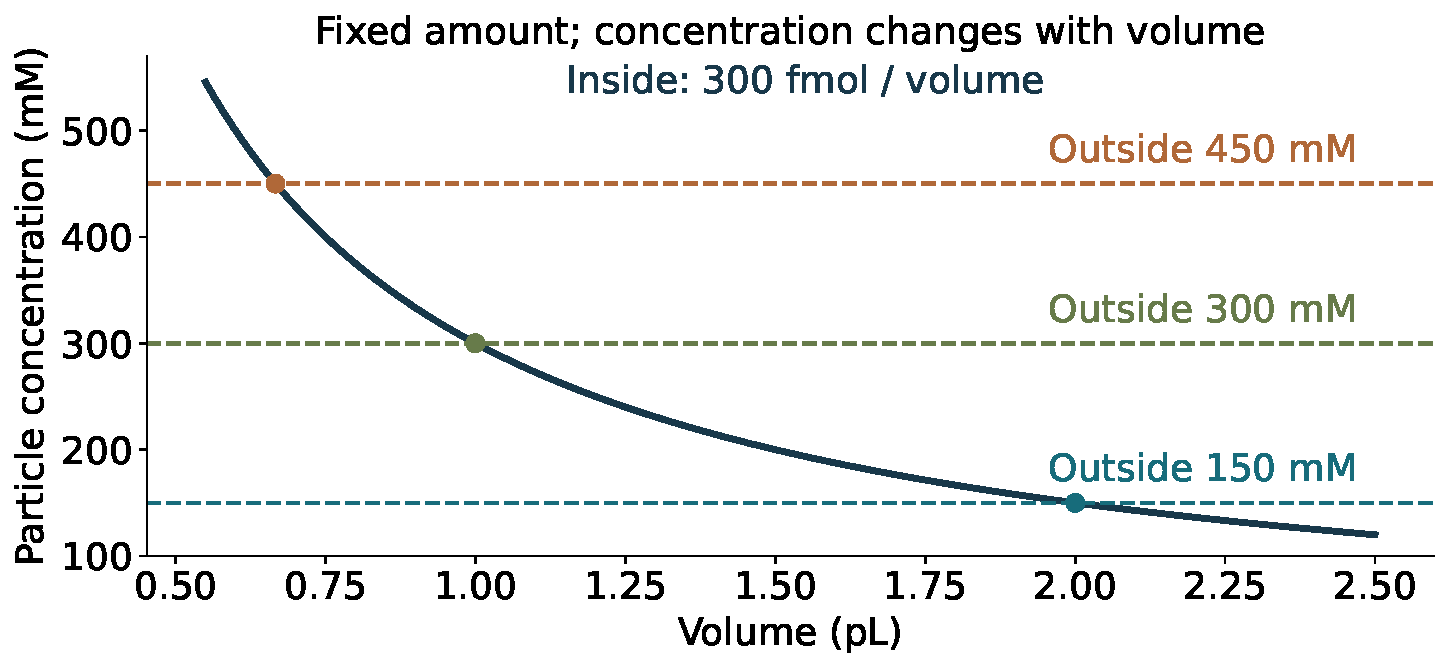
\includegraphics[width=.96\linewidth,height=.57\textheight,keepaspectratio]{osmotic-balance.pdf}\par\smallskip
{\small For 300 fmol of impermeant solute, c\_in =\allowbreak{} 300/V. Fixed external concentrations 150, 300 and 450 mM intersect at volumes 2, 1 and 2/3 pL under equal hydrostatic pressures.}
\end{minipage}\end{center}
\section{Dimensionless dynamics and an implicit exact solution}
\hypertarget{note-dimensionless-dynamics-and-an-implicit-exact-solution}{}\label{note:dimensionless-dynamics-and-an-implicit-exact-solution}
{\small \href{slides.html\#frame=a-common-dimensionless-equation\&step=1}{Slides for this section}}\par
Set $v=V/V_*$ and $\theta=t/\tau$, with the positive quantities defined above. Then
\[
\frac{\dd v}{\dd\theta}=\frac1v-1=\frac{1-v}{v}.
\]
All constant-parameter cases share this dimensionless equation. For a nonequilibrium initial value $v_0>0$, separate variables on its side of $v=1$:
\[
\theta=\int_{v_0}^{v}\frac{z}{1-z}\,\dd z
=v_0-v+\log\left|\frac{1-v_0}{1-v}\right|.
\]
The logarithm diverges as $v\to1$, expressing asymptotic approach. If $v_0=1$, use the constant solution instead; inserting it in the logarithmic expression would create an undefined ratio. This relation provides a reference for checking a numerical solution without introducing a second time-stepping method.

A useful dissipation function is
\[
\Phi(v)=v-1-\log v\geq0\quad(v>0).
\]
Its derivative is
\[
\frac{\dd\Phi}{\dd\theta}
=\left(1-\frac1v\right)\left(\frac1v-1\right)
=-\left(1-\frac1v\right)^2\leq0.
\]
Thus the dynamics decrease a nonnegative function whose unique minimum is equilibrium. This mathematical stability statement depends on the stated fixed-reservoir model.
\section{A volume update and its concentration consequence}
\hypertarget{note-a-volume-update-and-its-concentration-consequence}{}\label{note:a-volume-update-and-its-concentration-consequence}
{\small \href{slides.html\#frame=one-signed-flow-calculation\&step=1}{Slides for this section}}\par
Explicit Euler holds the starting flow fixed over a time interval $h$:
\[
V_{n+1}=V_n+hL(n/V_n-c_{\mathrm{out}}),\qquad
c_{n+1}=n/V_{n+1}.
\]
For $V_n=1\,\mathrm{pL}$, $n=300\,\mathrm{fmol}$, and $c_{\mathrm{out}}=150\,\mathrm{mM}$, the initial inflow is $0.002(300-150)=0.3\,\mathrm{pL/s}$. A $0.2$-second step gives $V_{n+1}=1.06\,\mathrm{pL}$ and $c_{n+1}=300/1.06\simeq283.019\,\mathrm{mM}$. It would be inconsistent to retain the old concentration after changing volume.

For shrinking states with $n/V_n<c_{\mathrm{out}}$, positivity requires
\[
h<\frac{V_n}{L(c_{\mathrm{out}}-n/V_n)}.
\]
Near equilibrium, Euler has perturbation multiplier $1-h/\tau$; $0<h/\tau<2$ gives local linear stability, while $h/\tau\leq1$ avoids local alternating overshoots. These are distinct from global accuracy. A step can produce a nonphysical overshoot even though the exact ODE is monotone. The supplied trajectories use $h=0.05$ seconds and reject inadmissible volumes; they do not silently clip them.
\begin{center}\begin{minipage}{.98\linewidth}\centering
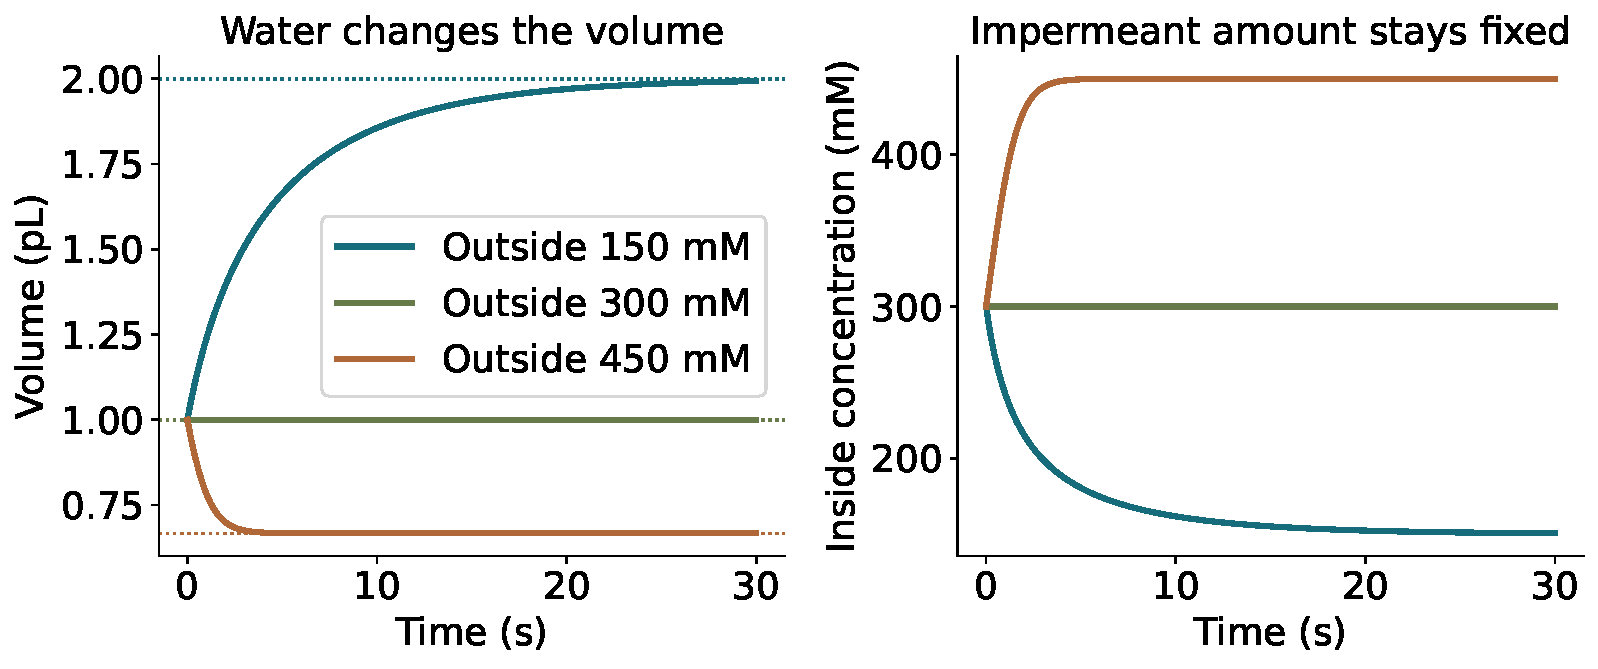
\includegraphics[width=.96\linewidth,height=.57\textheight,keepaspectratio]{volume-trajectories.pdf}\par\smallskip
{\small Synthetic explicit-Euler trajectories at step 0.05 s and L =\allowbreak{} 0.002 pL/(s mM). All start at 1 pL with 300 fmol trapped solute. Dotted lines show volume equilibria; survival and rupture are not modeled.}
\end{minipage}\end{center}
\section{Limiting cases and extension to volume regulation}
\hypertarget{note-limiting-cases-and-extension-to-volume-regulation}{}\label{note:limiting-cases-and-extension-to-volume-regulation}
{\small \href{slides.html\#frame=zero-external-concentration\&step=1}{Slides for this section}}\par
If $L=0$, no water moves and $V(t)=V_0$. If $c_{\mathrm{out}}=0$ with $L,n>0$, there is no finite equilibrium. The equation becomes $V\dot V=Ln$, giving
\[
V(t)=\sqrt{V_0^2+2Lnt}.
\]
This limiting solution is a useful independent numerical test. The model still does not predict a rupture threshold. Its unbounded growth simply records the absence of a balancing mechanism.

The source discussion of animal-cell volume regulation includes permeant ions and active transport. Our single-impermeant-solute experiment isolates the osmotic contribution and is not a reproduction of that full regulation model. Adding permeant species requires equations for their amounts as well as water volume; adding mechanical pressure requires a constitutive relation between pressure and geometry.

For the current companion, verify $n=c_{\mathrm{in}}V$, the equilibrium case, the sign of motion, and convergence under smaller steps. Compare $V(t)$ and $c(t)$ as coupled observables. A constant product checks bookkeeping; the implicit exact relation checks the trajectory. Neither demonstrates that a real cell has the chosen permeability or fixed external environment.
\bigskip
\section*{Exercises}
\par\noindent\begin{minipage}{\linewidth}
\subsection*{MM08-E1. Amount, concentration and one step}
Use n =\allowbreak{} 240 fmol, V0 =\allowbreak{} 0.80 pL, c\_out =\allowbreak{} 200 mM and L =\allowbreak{} 0.003 pL/(s mM).

\textbf{a} Compute initial inside concentration and inward-positive flow.

\end{minipage}\par\medskip
\textbf{b} Estimate V after 0.10 s with one explicit step; compute its concentration.

\textbf{c} Find equilibrium volume and explain what stays conserved during approach.

\par\noindent\begin{minipage}{\linewidth}
\subsection*{MM08-E2. Predict shrinking and separate timescale}
Use n =\allowbreak{} 360 fmol, V0 =\allowbreak{} 1.20 pL, c\_out =\allowbreak{} 450 mM and L =\allowbreak{} 0.002 pL/(s mM).

\textbf{a} Predict the initial direction and compute flow.

\end{minipage}\par\medskip
\textbf{b} Compute equilibrium volume. What changes if positive L doubles?

\textbf{c} What happens if L is instead exactly zero at the initial state?

\par\noindent\begin{minipage}{\linewidth}
\subsection*{MM08-E3. Check a conserved quantity}
A simulated compartment has fixed trapped amount 300 fmol.

\textbf{a} Find inside concentration at volumes 0.75 pL and 1.50 pL.

\end{minipage}\par\medskip
\textbf{b} A log reports V =\allowbreak{} 1.50 pL and c\_in =\allowbreak{} 250 mM. Is it consistent with the stated amount?

\textbf{c} Would constant total solute alone prove that a volume trajectory is accurate or biologically validated?

\par\noindent\begin{minipage}{\linewidth}
\subsection*{MM08-E4. Locate the model boundary}
Consider using the demonstration to predict what happens to an actual cell in a changed external solution.

\textbf{a} Name two mechanisms missing from the water-only model and a quantity each could alter.

\end{minipage}\par\medskip
\textbf{b} Explain why the computed volume 2 pL does not establish that a cell survives.

\textbf{c} Propose an observation and a numerical check for testing a volume-response explanation.

\section*{References}
\noindent\begin{minipage}{\linewidth}
Zan Ahmad, Fall 2024 HEART syllabus. PDF pages 1--2.

\end{minipage}\par\medskip
\noindent\begin{minipage}{\linewidth}
Hoppensteadt and Peskin, Modeling and Simulation in Medicine and the Life Sciences, second edition. Printed pages 109--115; PDF pages 122--128 in the supplied copy.

\end{minipage}\par\medskip
\end{document}
